\documentclass[letterpaper,11pt]{article}
\usepackage{graphicx}
\usepackage{listings}
\usepackage[super]{nth}
\usepackage[hyphens]{url}
\usepackage{amsmath}
\usepackage[makeroom]{cancel}
\usepackage[table]{xcolor}
\usepackage{comment}
\usepackage[space]{grffile}

\lstset{
	basicstyle=\footnotesize,
	breaklines=true,
}

\begin{document}

\begin{titlepage}

\begin{center}

\Huge{Assignment 7}

\Large{CS 595:  Introduction to Web Science}

\Large{Fall 2013}

\Large{Shawn M. Jones}

\Large Finished on \today

\end{center}

\end{titlepage}

\newpage
\section*{1}

\subsection*{Question}

\begin{verbatim}
1.  Using D3, create a graph of the Karate club before and after
the split.

- Weight the edges with the data from: 
http://vlado.fmf.uni-lj.si/pub/networks/data/ucinet/zachary.dat

- Have the transition from before/after the split occur on a mouse
click.
\end{verbatim}

\newpage
\subsection*{Answer}

The Karate club data has been rendered into graphs using D3 as shown in Figures \ref{fig:club-before} and \ref{fig:club-after}.  On load, the graph looks like Figure \ref{fig:club-before} and then looks like Figure \ref{fig:club-after} after a single click.  From that point, further clicks will toggle between the ``together'' Karate Club and the ``split'' Karate Club. A live version of this can be experienced at: \url{http://www.cs.odu.edu/~sjone/courses/cs595-ws-f13/graph.html}.

The code for generating the graph was shamelessly stolen from the D3 example at \url{http://bl.ocks.org/mbostock/950642} and is shown in Listing \ref{lst:q1codeHTML}.

From Listing \ref{lst:q1codeHTML}, the function \verb+loadgraph+ on line 42 does most of the work.  Line 43 shows the overall title of the graph being rendered.  Line 49 starts the loading of the appropriate JSON file and subsequent actions on that data.  Line 47 loads all of the edge data (referenced as \emph{links}) and line 63 loads all of the node data.  Line 69 inserts the image of the stick figures in for each person.  Line 76 appends the text labels to each node.  Line 81 actually draws the graph.

Line 104 sets up the canvas for the SVG code to populate, and line 109 starts the \emph{force directed layout}, which maps nodes to SVN \verb+<circle>+ elements and links to \verb+<line>+ elements.  Line 116 runs \verb+loadgraph+ for the first time.

All of that gets the graph drawn for the first time.  The click response is handled by the method referenced on line 107.  On a \verb+click+ event, the \verb+switchgraph+ function from line 27 is executed, which clears the existing graph and toggles the state, then calls load graph with the datafile and label associated with the set state.  The statement on line 35 allows the state to be toggled to the values defined on lines 96-100.

Of course, this just discusses the HTML/JavaScript/D3 part of the assignment.  The data set used was not in the JSON format, and hence had to be converted for use in D3.  Not wanting to use JavaScript to parse the file, I felt that this was a job for Python.

Listing \ref{lst:q1python1} shows the code that takes the given ``matrix'' dataset and converts it into JSON.  It is run like so:
\begin{lstlisting}[frame=single]
./convertdata.py | python -mjson.tool > club.json
\end{lstlisting}
The \verb+python -mjson.tool+ pretty formats the JSON code for human consumption.

Listing \ref{lst:q1python2} shows the code that takes the JSON produced by \verb+convertdata.py+ and runs the Girvan-Newman algorithm over it, splitting the graph into two clusters.  It is run like so:
\begin{lstlisting}[frame=single]
./createClubSplit.py club.json > split-club.json
\end{lstlisting}
This time, I natively pretty formatted the output with line 35.

Thus, the Python programs \verb+convertdata.py+ and \verb+createClubSplit.py+ create the JSON files that are consumed by the JavaScript in \verb+graph.html+.

\clearpage
\begin{figure}[h]
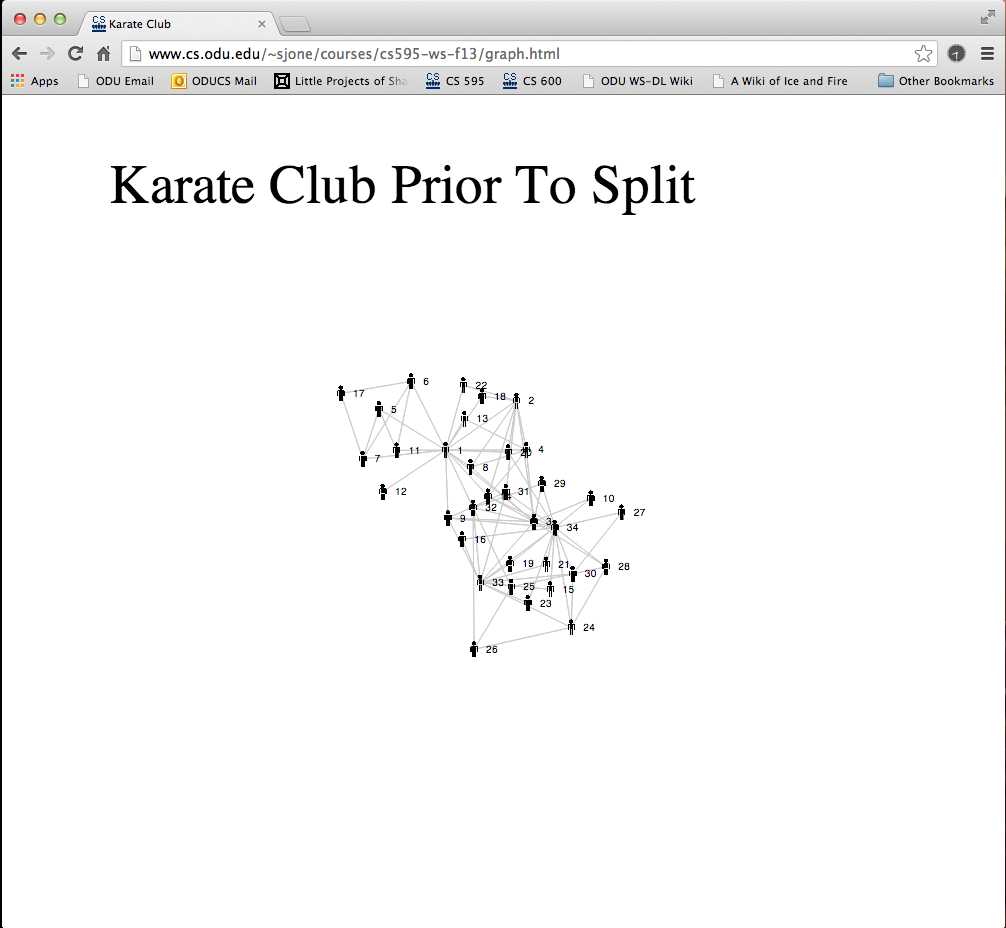
\includegraphics[scale=0.4]{club-before-screenie.png}
\caption{Screenshot of Karate Club Graph Before Split Drawn in D3}
\label{fig:club-before}
\end{figure}

\clearpage
\begin{figure}[h]
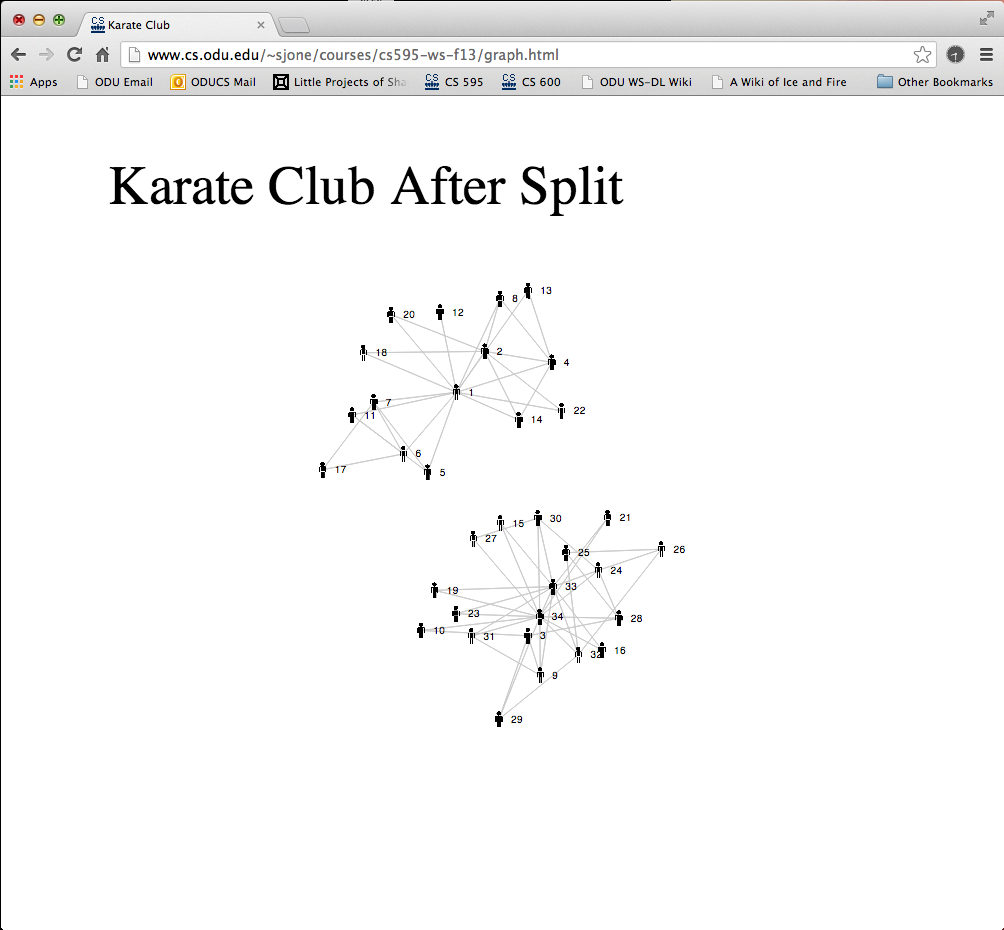
\includegraphics[scale=0.4]{club-after-screenie.png}
\caption{Screenshot of Karate Club Graph Split Drawn in D3}
\label{fig:club-after}
\end{figure}

\clearpage
\lstinputlisting[language=html,frame=single,caption={HTML/JavaScript code that displays the graphs shown in the screenshots from Figures \ref{fig:club-before} and \ref{fig:club-after}},label=lst:q1codeHTML,captionpos=b,numbers=left,showspaces=false,showstringspaces=false,basicstyle=\footnotesize]{q1/graph.html}

\clearpage
\lstinputlisting[language=python,frame=single,caption={Python code that converts the given matrix data file into JSON for the initial ``together'' view of the Karate Club that is used for the graph shown in Figure \ref{fig:club-before}},label=lst:q1python1,captionpos=b,numbers=left,showspaces=false,showstringspaces=false,basicstyle=\footnotesize]{q1/convertdata.py}

\clearpage
\lstinputlisting[language=python,frame=single,caption={Python code that takes in the code produced by Listing \ref{lst:q1python1}, runs the Girvan-Newman algorithm on it, and then produces a JSON file showing the split Karate Club to be used by the graph shown in Figure \ref{fig:club-after}},label=lst:q1python1,captionpos=b,numbers=left,showspaces=false,showstringspaces=false,basicstyle=\footnotesize]{q1/createClubSplit.py}


\newpage

\section*{2}

\subsection*{Question}

\begin{verbatim}
2.  Use D3 to create a who-follows-whom graph of your Twitter
account.  Use my twitter account ("@phonedude_mln") if you do not
have an interesting number of followers.
\end{verbatim}

\subsection*{Answer}

Not attempted


\clearpage
\bibliographystyle{acm}
\bibliography{references}

\end{document}